%Preamble
\documentclass{article}
\usepackage{hyperref}
\usepackage[
    type={CC},
    modifier={by-nc-sa},
    version={3.0},
]{doclicense}
\usepackage[landscape]{geometry}
\usepackage{url}
\usepackage{multicol}
\usepackage{amsmath}
\usepackage{dsfont}
\usepackage{esint}
\usepackage{amsfonts}
\usepackage{tikz}
\usetikzlibrary{decorations.pathmorphing}
\usepackage{amsmath,amssymb}

\usepackage{siunitx}

\usepackage{colortbl}
\usepackage{xcolor}
\usepackage{mathtools}
\usepackage{amsmath,amssymb}
\usepackage{enumitem}
\makeatletter

\newcommand*\bigcdot{\mathpalette\bigcdot@{.5}}
\newcommand*\bigcdot@[2]{\mathbin{\vcenter{\hbox{\scalebox{#2}{$\m@th#1\bullet$}}}}}
\makeatother

\title{PHYS 250 Formula Sheet}
\usepackage[english]{babel}
\usepackage[utf8]{inputenc}

\renewcommand{\baselinestretch}{1.15}

\advance\topmargin-.8in
\advance\textheight3in
\advance\textwidth3in
\advance\oddsidemargin-1.5in
\advance\evensidemargin-1.5in
\parindent0pt
\parskip2pt
\newcommand{\hr}{\centerline{\rule{3.5in}{1pt}}}
\newcommand\subtopic[1]{
    \textbf{#1}
    \vspace{.1cm}
    \hrule
    \vspace{.2cm}}
%\colorbox[HTML]{e4e4e4}{\makebox[\textwidth-2\fboxsep][l]{texto}

% Definitions for shortcuts
\newcommand{\ih}{\hat{i}}
\newcommand{\jh}{\hat{j}}
\newcommand{\kh}{\hat{k}}
\newcommand{\uh}{\hat{u}}
\newcommand{\vx}{\vec{x}}
\newcommand{\vy}{\vec{y}}
\newcommand{\vz}{\vec{z}}
\newcommand{\vr}{\vec{r}}
\newcommand{\vs}{\vec{s}}
\newcommand{\vv}{\vec{v}}
\newcommand{\va}{\vec{a}}
\newcommand{\vF}{\vec{F}}
\newcommand{\vE}{\vec{E}}
\newcommand{\fvec}[1]{\underrightarrow{#1}}
\newcommand{\f}{\mathrm{f}}
\newcommand{\Ra}{\Rightarrow}
\newcommand{\brangle}[1]{\left\langle #1 \right\rangle}
\newcommand{\brround}[1]{\left( #1 \right)}
\newcommand{\brcurly}[1]{\left\{ #1 \right\}}
\newcommand{\brsquare}[1]{\left[ #1 \right]}
\newcommand{\brvertical}[1]{\left| #1 \right|}
\newcommand{\matrixx}[1]{\left[\begingroup        \renewcommand{\arraystretch}{1}\begin{matrix} #1 \end{matrix}\endgroup\right]}
\newcommand{\eqnsystem}[1]{\left\{\begin{matrix} #1 \end{matrix}\right.}
\newcommand{\detmatrix}[1]{\left|\begin{matrix} #1
\end{matrix}\right|}
\newcommand{\R}{\mathds{R}}
\newcommand{\Z}{\mathds{Z}}
\newcommand{\N}{\mathds{N}}
\newcommand{\eval}[1]{\left. #1 \right|}
\newcommand{\augmatrix}[2]{\left[\begin{array}{#1|c}#2\end{array}\right]}
\newcommand{\lap}[1]{\Lap\brcurly{#1}}
\newcommand{\ilap}[1]{\Lap^{-1}\brcurly{#1}}
\newcommand{\para}{\parallel}
\newcommand{\formula}[2]{\begin{center} \begin{tcolorbox}[text width = #1] $$#2$$\end{tcolorbox}\end{center}}

% New Command added by SG for partial derivatives
% \pder[f]{x} and \pder{x} to use with 1 or two args
\newcommand{\pder}[2][]{\frac{\partial#1}{\partial#2}}

%New operators
\DeclareMathOperator{\arccot}{arccot}
\DeclareMathOperator{\arccsc}{arccsc}
\DeclareMathOperator{\arcsec}{arcsec}
\DeclareMathOperator{\sgn}{sgn}
\DeclareMathOperator{\Ai}{Ai}


\begin{document}

\begin{center}{\huge{\textbf{PHYS 250 - Unofficial Formula Sheet}}}\\
\end{center}
\begin{multicols*}{2}

\tikzstyle{mybox} = [draw=black, fill=white, very thick,
    rectangle, rounded corners, inner sep=10pt, inner ysep=10pt]
\tikzstyle{fancytitle} =[fill=black, text=white, font=\bfseries]

\renewcommand{\arraystretch}{1.7}

\small

%------------ Relativity ---------------
\begin{tikzpicture}
\node [mybox] (box){%
    \begin{minipage}{0.45\textwidth}
    \subtopic{Lorentz Transformations}
    \begin{tabular}{lp{8cm} l}
        Beta & $\beta = \frac{u}{c} = \frac{x'}{t'c}$\\
        Gamma & $\gamma = \frac{1}{\sqrt{1-(\frac{u}{c})^2}}$\\
        Transforms & $x'=\gamma(x-\beta ct)$\\
         & $ct'=\gamma(ct-\beta x)$\\
        Inverse Transforms & $x=\gamma(x'+\beta ct')$\\
         & $ct=\gamma(ct'+\beta x')$
    \end{tabular}\\
    \subtopic{Lorentz Contractions}
    \begin{tabular}{lp{8cm} l}
        Length Contraction & $L_{\text{moving}}=\frac{L_{\text{rest}}}{\gamma}$\\
        Time Dilation & $T_{\text{moving}}=\gamma T_{\text{rest}}$\\
        Doppler Effect & $f_{\text{obs}}=f_{\text{source}}\sqrt{\frac{1-\beta}{1+\beta}} = f_{\text{source}}\sqrt{\frac{c+u}{c-u}}$\\
        & $\Delta T_{obs}=\Delta T_{\mathrm{source}}\frac{\sqrt{1+\beta}}{\sqrt{1-\beta}}$\\
        & $\lambda_{_\mathrm{obs}}=\lambda_{_\mathrm{source}}{\frac{\sqrt{1+\beta}}{\sqrt{1-\beta}}}$\\
        & $\beta > 0$ when source and observer are moving apart \\

        Velocity Addition & $v_{\text{rel}}=\frac{v'+u}{1+\frac{v'u}{c^2}}, \ \beta = \frac{\beta_1+\beta_2}{1+\beta_1\beta_2}$
    \end{tabular}
    \end{minipage}
};
%------------ Relativity ---------------------
\node[fancytitle, right=10pt] at (box.north west) {Relativity};
\end{tikzpicture}

%------------ Photons ---------------
\begin{tikzpicture}
\node [mybox] (box){%
    \begin{minipage}{0.45\textwidth}
    \begin{tabular}{lp{8cm} l}
        Planck-Einstein & $E=hf=\frac{hc}{\lambda}$\\
        Einstein photoelectric & $E_{max}=hf-\phi q$\\
        X-ray tube spectrum & $\lambda_{min}=\frac{hc}{E_{\text{electron}}}=\frac{hc}{\text{qV}}$\\
        Stopping Potential & $V_{stop}=\frac{hf}{q}-\phi_{work}$\\
        Bragg's Law & $2d\sin(\theta_{\text{surface}})=n\lambda\quad d=\text{spacing}$\\
        Compton Scattering & $\lambda^{\prime}\!-\!\lambda=\!\frac{h}{m c}\!\left(1\!-\!\cos\theta\right)\ \ \frac{h}{m c}\!=\!2.426\ \mathrm{pm}$
        \\
        Photon Polarization &
        $\text{Prob} = \cos^2{\phi}\quad\phi=\text{angle between polarization}$
        \\
        Blackbody Spectrum & $dI=\frac{2hf^3}{c^2}\cdot\frac{1}{e^{\frac{hf}{kT}}-1}\cdot df$
        \\
    \end{tabular}\\
    \end{minipage}
};
\node[fancytitle, right=10pt] at (box.north west) {Photons};
\end{tikzpicture}

\vfill\null
\columnbreak

%------------ Constants ---------------
\begin{tikzpicture}
\node [mybox] (box){%
    \begin{minipage}{0.45\textwidth}
    \begin{multicols}{2}
    $\qty{1}{\electronvolt} = \qty{1.602e-19}{\joule}$\\
    $c=\qty{2.998e8}{\meter\per\second}$\\
    $h=\qty{6.626e-34}{\joule\second}=\qty{4.135e-15}{\electronvolt\second}$\\
    $hc=\qty{1240}{\electronvolt\nano\meter}=\qty{1.986e-25}{\joule\meter}$
    \\
    $q = \qty{1.602e-19}{\coulomb}$\\
    $\hbar=\frac{h}{2\pi}=\qty{1.055e-34}{\joule\second}$\\
    $\hbar=\qty{6.5821e-16}{\electronvolt\second}$\\
    $m_e=\qty{9.11e-31}{kg}=\qty{5.11e5}{\electronvolt}/c^2$
    $\epsilon_0=\qty{8.854e-12}{\farad\per\meter}$
    \end{multicols}
    \end{minipage}
};
\node[fancytitle, right=10pt] at (box.north west) {Constants};
\end{tikzpicture}

%------------ Relativistic Momentum ---------------
\begin{tikzpicture}
\node [mybox] (box){%
    \begin{minipage}{0.45\textwidth}

    
    \subtopic{Spacetime 4-Vector and Invariance}
    Observers in different reference frames may disagree on order events, and/or their spatial relation, but the length of the spacetime 4-vector and its dot products is invariant (same for all observers):
    \begin{align*}
    \text{Definition}: && \underbrace{\fvec{X}}_{\text{Space-time}} &= \quad \langle\underbrace{ct}_{\text{Observer's time}}, \underbrace{\vec{x}}_{\text{Distance from Observer}}\rangle\\
    \text{Properties}: && \fvec{X}\cdot \fvec{Y} &= \fvec{X}' \cdot \fvec{Y}' = c^2t_x\cdot t_y - \vec{x}\cdot \vec{y}
    \end{align*} 
    
    Note that 'proper time' $\tau$, the passage of time for the moving object's frame of reference, is also the same for all observers.  Relativistic energy and momentum are intertwined through spacetime, it is their sum that is conserved:
    \vspace{-.3cm}
    \begin{align*}
    \text{Spacetime Energy-Momentum}: && \fvec{P} &= m\frac{d}{d\tau}\fvec{X} = \brangle{\frac{E_{rel}}{c},\vec{p}}\\
    \text{Energy-Momentum Invariance}: && \fvec{P}\cdot \fvec{P} &= \fvec{P}' \cdot \fvec{P}' = \frac{1}{c^2}(E^2 - |\vec{p}|^2c^2)
    \end{align*} 
    
    \subtopic{Momentum and Energy}
    \begin{tabular}{rp{8cm} l}
        Relativistic Momentum & $\vec{p} = \frac{m\vec{v}}{\sqrt{1-v^2/c^2}} = \gamma m\vec{v}$\\
        Kinetic Energy & $K = \frac{mc^2}{\sqrt{1-v^2/c^2}}-mc^2 = (\gamma -1)mc^2$\\
        Net Energy & $E = K+mc^2 = \gamma m c^2$\\
          & $E^2=(mc^2)^2+(pc)^2$\\
        Along Particle Path & $p_{decay} = \gamma p' +\beta \gamma E'$\\
        
    \end{tabular}\\
        \subtopic{Center of Mass}
    \begin{tabular}{rp{8cm} l}
        General Center of Mass & $\vec{p}_1+\vec{p}_2=\vec{0}$\\
        & $\brround{\frac{E_1+E_2}{c}}^2=\brround{\frac{E_{CM}}{c}}^2=(m_1c)^2+\fvec{P}_1\cdot\fvec{P}_2+(m_2c)^2$\\
        Beam and Particle at Rest & $\brround{\frac{E_{CM}}{c}}^2=(m_1c)^2+2m_2E_{1\text{ lab}}+(m_2c)^2$\\
        Particle Decay & $\brround{\fvec{P}_0}^2=(m_0c)^2=(\fvec{P}_1+\fvec{P}_2)^2=\brangle{\frac{E_1+E_2}{c},\vec{p}_1+\vec{p}_2}^2$
    \end{tabular}
    \end{minipage}
};
%------------ Relativity ---------------------
\node[fancytitle, right=10pt] at (box.north west) {Relativistic Momentum};
\end{tikzpicture}


 

%------------ Atoms and Bohr ---------------
\begin{tikzpicture}
\node [mybox] (box){%
    \begin{minipage}{0.45\textwidth}
    \subtopic{Constants}
    $B=\qty{364.5}{\nano\meter}$ for Hydrogen\\
    $R=\frac{4}{B}=\qty{1.097e7}{\per\meter}$\\
    \subtopic{Equations}
    \begin{tabular}{lp{8cm} l}
    Angular Momentum & $L=n\hbar$\\
    Diffraction & $sin\theta = n\frac{\lambda}{d}, \text{if } d\gg\lambda \text{ diffraction is invisible}$\\
    Improved Balmer & $\lambda = B\frac{n^2}{n^2-m^2},\ n>m$\\
    & \begin{tabular}{cl}
        \vspace{-0.35cm}
        $m=1$: & Lyman (UV)\\
        \vspace{-0.35cm}
        $m=2$: & Balmer (visible)\\
        \vspace{-0.35cm}
        $m=3$: & Paschen (IR)
    \end{tabular}\\
    Improved Rydberg & $\frac{1}{\lambda} = RZ^2(\frac{1}{n^2_1}-\frac{1}{n^2_2}) \text{ with } n_2 > n_1$\\
    Photon Energy & $E = \qty{13.6}{\electronvolt}\cdot Z^2(\frac{1}{n^2_1}-\frac{1}{n^2_2})$\\
    Rutherford Orbit Energy & $E_\text{total} = -\frac{qQ}{8\pi \epsilon_0 r} = -\frac{m}{2}\brround{\frac{qQ}{4\pi \epsilon_0}}^2\frac{1}{L^2}$\\
    Rutherford Atomic Decay & $t_\text{seconds}=39.2\, \mathrm{ns}\cdot|E_\text{eV}|^{-3}$\\
    Bohr Atomic Energy & $E = -\frac{m}{2}\brround{\frac{q^2}{4\pi\epsilon_0 \hbar}}^2\frac{Z^2}{n^2}=\qty{-13.6}{\electronvolt}(\frac{Z^2}{n^2})$\\
    Bohr Model Radius & $r = \frac{4\pi\epsilon_0\hbar^2n^2}{Zmq^2}=\frac{q^2Z}{8\pi\epsilon_0 E}=52.97\, \mathrm{pm}(\frac{n^2}{Z}$)\\
    Bohr Orbit Velocity & $v=\frac{Zq^2}{L4\pi\epsilon_0}=\frac{Zq^2}{4\pi\epsilon_0 n\hbar}$\\
    & $\beta=\frac{v}{c}=7.293\cdot 10^{-3}(\frac{Z}{n})$\\
    Moseley's Law (X-Ray Emission) & $E = \qty{13.6}{\electronvolt}\left(\frac{1}{n_1^2}-\frac{1}{n_2^2}\right)\cdot(Z-b)^2$\\
    & \begin{tabular}{cl}
        \vspace{-.35cm}
        $\mathrm{K\alpha}$: $b = 1, n_1 = 1, n_2 =2$\\
        \vspace{-.35cm}
        $\mathrm{K\beta}$: $b = 1, n_1=1, n_2 = 3$\\
        \vspace{-.35cm}
        $\mathrm{L\alpha}$: $b=7.4, n_1=2, n_2=3$
    \end{tabular}\\
    de Broglie Wavelength & $\lambda_\text{electron} =  \frac{1.227\sqrt{\mathrm{eV}}\cdot \mathrm{nm}}{\sqrt{E_\text{electron}}}$\\
    & $\lambda_\text{matter} = \frac{h}{p}= \frac{hc}{\sqrt{2mc^2E_\text{kinetic}}}$\\
    Reduced Mass & $\mu=\frac{m_em_X}{m_e+m_X}$, $X$ is mass of nucleus
    \end{tabular}
    \end{minipage}
};
\node[fancytitle, right=10pt] at (box.north west) {Atoms and Bohr};

\end{tikzpicture}

%------------ Atoms and Bohr ---------------
\begin{tikzpicture}
\node [mybox] (box){%
    \begin{minipage}{0.45\textwidth}
    \subtopic{We love lasers}
    \begin{tabular}{lp{8cm} l}
Spontaneous emissions per second & $\frac{N}{\tau}$ where $\tau$ is the lifetime\\
Law of collisions & $\rho\sigma\lambda=1$ \scriptsize where $\sigma$ is collision cross section per atom\\
\scriptsize Number of photons after travelling distance & $N(x)=N_0e^{-\frac{x}{\lambda}}$
    \end{tabular}
    \end{minipage}
};
\node[fancytitle, right=10pt] at (box.north west) {LAZERS!};

\end{tikzpicture}

%------------ Schrodinger Wavefunctions ---------------
\begin{tikzpicture}
\node [mybox] (box){%
    \begin{minipage}{0.45\textwidth}
    \subtopic{Wave Equation}
    \begin{tabular}{lp{8cm} l}
Schrodinger Equation & $i\hbar\frac{\partial\Psi}{\partial t}=\hat{H}\Psi=-\frac{\hbar^2}{2m}\frac{\partial^2\Psi}{\partial x^2}+V(x)\Psi$\\
Angular Frequency & $\omega = \frac{2\pi}{T}=2\pi f$\\
Energy & $E_K=hf=\hbar\omega=\frac{1}{2}mv^2=\frac{p^2}{2m}$\\
Momentum & $p=\hbar k$\\
Free Particle Solutions & $\Psi(x,t) = A\sin\brround{\pm kx-\omega t + \phi},\ k = \frac{2\pi}{\lambda}$\\
 & $\Psi(x,t)=e^{i(kx-\omega t)} = e^{i\frac{px-Et}{\hbar}}$
\end{tabular}
\subtopic{Operators}
\begin{tabular}{lp{8cm} l}
Momentum Operator & $\hat{p}\Psi=-i\hbar\frac{\partial}{\partial x}\Psi$\\
Hamiltonian Operator & $\hat{H}\Psi=\frac{\hat{p}^2}{2m}\Psi+V\Psi=-\frac{\hbar^2}{2m}\Psi+V\Psi$
  \end{tabular}
\subtopic{Probability Density}
\begin{tabular}{lp{3cm} l}
Probability Density & $\rho(x)=\Psi^*\Psi$ & $\int_{-\infty}^\infty \Psi^*\Psi dx=1$\\
Normalized Gaussian & $f(x)=\frac{1}{\sqrt{2\pi\sigma^2}}e^{-\frac{x^2}{2\sigma^2}}$\\
Transformed Gaussian & $\sigma_x\sigma_k=1$\\
Heisenberg Uncertainty Principle & $\sigma_x\sigma_p\geq\frac{\hbar}{2}$
\end{tabular}
\subtopic{Schrodinger PDEs}
\begin{tabular}{lp{8cm} l}
TISE & $-\frac{\hbar^2}{2m}\frac{\partial^2\psi}{\partial x^2}+V(x)\psi=E\psi$\\
Time Dependent Solution & $\varphi(t)=e^{-\frac{iE_n}{\hbar}t}$\\
Solution to Schrodinger & $\Psi_n(x,t)=\psi_n(x)\varphi_n(t)=\psi_n(x)e^{-\frac{iE_n}{\hbar}}$
\end{tabular}
    \end{minipage}
};
\node[fancytitle, right=10pt] at (box.north west) {Basics of Quantum Mechanics};

\end{tikzpicture}


%-------------------Authorship-----------------------
\begin{center}
    \framebox{
    \parbox[t][1.0cm]{8.5cm}{
    \addvspace{0.2cm} \centering 
    \footnotesize Compiled by Tyler Wilson, Alex Koen, Ethan Predinchuk, Spencer Bradbury, and Simon Ghyselincks 2022
    } 
}
\end{center}
\newpage


%------------ Schrodinger Potential Barriers/Wells ---------------
\begin{tikzpicture}
\node [mybox] (box){%
    \begin{minipage}{0.45\textwidth}
    \subtopic{Step Potentials}
    \begin{tabular}{l l l}
Wavefunctions & $\begin{cases}\psi_I=e^{ikx} & \text{(Incident)}\\ \psi_R=Re^{-ikx} & \text{(Reflected)}\\ \psi_T=Te^{ik'x} & \text{(Transmitted)}\end{cases}$\\
Wavenumbers & $k=\frac{\sqrt{2mE}}{\hbar}$ & $k'=\frac{\sqrt{2m(E-V)}}{\hbar}$\\
Amplitudes & $R=\frac{k-k'}{k+k'}$ & $T=\frac{2k}{k+k'}$\\
Flux & $\Phi=\text{density}\cdot\text{velocity}$\\
Incident Flux & $\Phi_I=\frac{\hbar k}{m}$ & $\Phi_I=\Phi_R+\Phi_T$\\
Reflected Flux & $\Phi_R=\frac{\hbar k}{m}R^2=\frac{\hbar k}{m}\brround{\frac{k-k'}{k+k'}}^2$\\
Transmitted Flux & $\Phi_T=\frac{\hbar k'}{m}T^2=\frac{\hbar k'}{m}\brround{\frac{2k}{k+k'}}^2$\\
Probability & $P(R)=\frac{\Phi_R}{\Phi_I}=R^2$ & $P(T)=\frac{\Phi_T}{\Phi_I}=\frac{k'}{k}T^2$
\end{tabular}\\
    \subtopic{Potential Barriers}
    \begin{tabular}{lp{8cm} l}
Wavefunctions & $\begin{cases} \psi_I=e^{ikx} & \text{(Incident)}\\ \psi_R=Re^{-ikx} & \text{(Reflected)}\\ \psi_T=Te^{ikx} & \text{(Transmitted)}\\ \psi_F=Fe^{ik'x} & \text{(Forward)}\\ \psi_B=Be^{-ik'x} & \text{(Backward)} \end{cases}$\\
Amplitudes & $\matrixx{-1 & 1 & 1 & 0 \\ k & k' & -k' & 0 \\ 0 & e^{ik'w} & e^{-ik'w} & -e^{ikw} \\ 0 & k'e^{ik'w} & -k'e^{-ik'w} & -ke^{ikw}}\matrixx{R\\F\\B\\T}=\matrixx{1\\k\\0\\0}$\\
Approximate Tunneling & $P(T)\approx16\frac{E}{V}\brround{1-\frac{E}{V}}e^{-2\kappa l},\ \kappa=\frac{\sqrt{2m(V-E)}}{\hbar}$, $l$ is length
\end{tabular}
\subtopic{Infinite Square Well}
    \begin{tabular}{lp{8cm} l}
Energy & $E_n=-\frac{\hbar^2\pi^2n^2}{2mw^2}$, $w$ is width\\
Inside Wavefunction & $\psi_n(x)=\sqrt{\frac{2}{w}}\sin(k_n x),\ k_n=\frac{n\pi}{w}$\\
Outside Wavefunction & $\psi_n(x) = e^{\pm k'x}, \ k_n' = \frac{n\pi}{w}$
\end{tabular}\\
\subtopic{Finite Potential Wells}
    \begin{tabular}{lp{8cm} l}
Energy & $E_n<\frac{\hbar^2\pi^2n^2}{2mw^2}-V<0,\ E>0$\\
Wavefunction Inside & $\psi_n(x)=A\sin(kx)+B\cos(kx),\ k=\sqrt{\frac{2mE}{\hbar^2}}$\\
Wavefunction Outside & $\psi_n(x)=Ce^{k'x}+De^{-k'x},\
k'=\sqrt{\frac{2m(V-E)}{\hbar^2}}$,\\
\end{tabular}
    \end{minipage}
};
\node[fancytitle, right=10pt] at (box.north west) {Step Potentials, Barriers, and Wells};

\end{tikzpicture}

%------------ Schrodinger Potential Barriers/Wells ---------------
\begin{tikzpicture}
\node [mybox] (box){%
    \begin{minipage}{0.45\textwidth}
    \subtopic{Linear Potentials $V(x)=Fx$}
    \begin{tabular}{lp{8cm} l}
Airy Equation & $\frac{\partial^2y}{\partial x^2} = xy,\ x>0\Ra \Ai(x) \approx 0.35503e^{-x^{1.25}}$ \\ 
& $x < 0\Ra \Ai(x)\approx 0.56417 |x|^{-0.25}\sin\brround{\frac{|x|^{1.5}}{1.5} + \frac{\pi}{4}}$\\
& $ x \to x+E/F \text{ so } \frac{\partial^2\psi}{\partial x^2} = \frac{Fx}{\hbar^2/2m}\psi$\\
$\Ai(x)$ roots & $|\text{roots}|=-2.33811,–4.08795,–5.52056,-6.78671$\\ & $|\text{roots}|\approx-((n-\frac{1}{4})1.5\pi)^{2/3}$\\
Energy & $E = (\frac{\hbar^2F^2}{2m})^{1/3}\cdot|\text{roots}|$
\end{tabular}\\
\subtopic{Quantum Harmonic Oscillator $V(x)=\frac{1}{2}kx^2$}
    \begin{tabular}{lp{8cm} l}
Energy & $E_n=\frac{2n+1}{2}\hbar\sqrt{\frac{k}{m}}=\frac{2n+1}{2}\hbar\omega_\text{classical}$\\
Wavefunction & $\psi_n(x)=H_n\brround{\frac{x}{b}}e^{-\frac{x^2}{2b^2}}$\\
Terms & $ b^2 = (2\sigma)^2 = \frac{\hbar}{\sqrt{km}},\ \omega_\text{classical} = \sqrt{\frac{k}{m}}$\\
Hermite Polynomials & $\begin{cases}
H_0(x) = 1 \\
H_1(x) = 2x\\
H_2(x) = 4x^2-2\\
H_3(x) = 8x^3 - 12x\\
H_4(x) = 16x^4 - 48x^2 + 12\\
H_5(x) = 32x^5 - 160x^3 + 120x\\
H_6(x) = 64x^6 - 480x^4 + 720x^2 - 120\\
H_7(x) = 128x^7 - 1344x^5 + 3360x^3 - 1680\\
H_8(x) = 256x^8 - 3584x^6 + 13440x^4 - 13440x^2 + 1680
\end{cases}$
\end{tabular}
    \end{minipage}
};
\node[fancytitle, right=10pt] at (box.north west) {Real Potentials};

\end{tikzpicture}


%------------ Schrodinger Potential Barriers/Wells ---------------
\begin{tikzpicture}
\node [mybox] (box){%
    \begin{minipage}{0.45\textwidth}
\subtopic{Free Particle}
    \begin{tabular}{lp{8cm} l}
Wavefunction & $\Psi(\vec{x},t)=e^{i(\vec{k}\cdot\vec{x}-\omega t)}$\\
Energy & $E=\frac{\vec{p}^2}{2m}=\frac{(\hbar^2\vec{k})^2}{2m}=\hbar\omega$
\end{tabular}\\
\subtopic{Particle in a Box ($0<x<a,\ 0<y<b,\ 0<z<c$)}
    \begin{tabular}{lp{8cm} l}
Wavefunction & $\psi_{n_x,n_y,n_z}(\vec{x})=\sin\brround{\frac{n_x\pi x}{a}}\sin\brround{\frac{n_y\pi y}{b}}\sin\brround{\frac{n_z\pi z}{c}}$\\
Energy & $E_{n_x,n_y,n_z}=\brround{\frac{n_x^2}{a^2}+\frac{n_y^2}{b^2}+\frac{n_z^2}{c^2}}\frac{\hbar^2\pi^2}{2m},\ n>0$\\
Energy in a Cube & $E_{n_x,n_y,n_z}=\brround{n_x^2+n_y^2+n_z^2}\frac{\hbar^2\pi^2}{2mw^2},\ n>0$
\end{tabular}
    \end{minipage}
};
\node[fancytitle, right=10pt] at (box.north west) {Schrodinger in 3D};

\end{tikzpicture}


%------------ Schrodinger Potential Barriers/Wells ---------------
\begin{tikzpicture}
\node [mybox] (box){%
    \begin{minipage}{0.45\textwidth}
\subtopic{General Spherical Relationships}
    \begin{tabular}{lp{8cm} l}
    \vspace{-0.2cm}
Spherical Laplacian & $\nabla^2\Psi=\frac{1}{r^2}\frac{\partial}{\partial r}\brround{r^2\frac{\partial \Psi}{\partial r}}+\frac{1}{r^2\sin\theta}\frac{\partial}{\partial \theta}\brround{\sin\theta\frac{\partial\Psi}{\partial\theta}}+\frac{1}{r^2\sin^2\theta}\frac{\partial^2\Psi}{\partial\phi^2}$\\
\vspace{-0.2cm}
Separable Functions & $\Psi(r,\theta,\phi)=F(r)G(\theta)H(\phi)$\\
\vspace{-0.2cm}
Equations & $\begin{cases}\frac{\partial^2H(\phi)}{\partial\phi^2} = -\mu H(\phi)\\
\sin(\theta)\frac{\partial}{\partial\theta}\brround{sin\theta \frac{\partial G(\theta)}{\partial\theta}} = \brround{\mu - \lambda sin^2\theta}G(\theta)\\
-\frac{\hbar^2}{2M}\frac{\partial^2U(r)}{\partial r^2}+[V(r)+\frac{\hbar^2\lambda}{2Mr^2}]U(r) = E\cdot U(r)
\end{cases}$\\
\vspace{-0.2cm}
$\phi$ dependent & $H(\phi)=e^{im\phi},\ m\in\Z$\\
\vspace{-0.2cm}
$\theta$ dependent & $G(\theta)=P_\ell^m(\theta)$ (the associated Legendre functions)\\
\vspace{-0.2cm}
$r$ dependent & $F(r)=\frac{1}{r}U_{k\ell}(r)$\\
\vspace{-0.2cm}
Spherical Harmonics & $Y_\ell^m(\theta,\phi)=P_\ell^m(\theta)e^{im\phi}$
\end{tabular}\\
\begin{center}
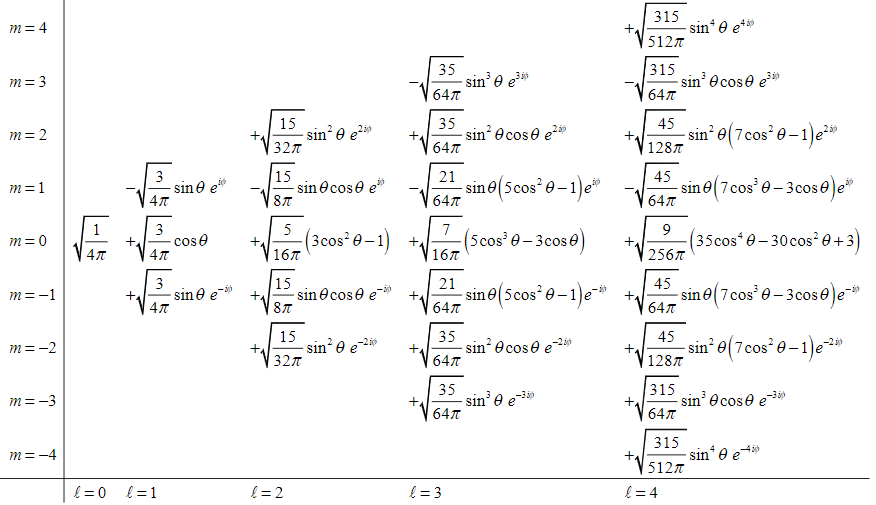
\includegraphics[scale=0.6]{SphericalHarmonics.png}
\end{center}
    \begin{tabular}{lll}
$m=\brcurly{\cdots,-2,-1,0,1,2,\cdots}$ & $\ell=\brcurly{0,1,2,\cdots}$ & $|m|\leq\ell$
\end{tabular}\\
$|m|$ is the power of $\sin\theta$ and $\ell$ is the power of $\sin\theta$ plus the highest power of $\cos\theta$\\
    \begin{tabular}{lp{8cm} l}
General Solution & $\psi_{k\ell m}(r,\theta,\phi)=\frac{1}{r}U_{k\ell}(r)Y_\ell^m(\theta,\phi)$
\end{tabular}\\
\subtopic{Infinite Spherical Square Well}
    \begin{tabular}{lp{8cm} l}
Energy & $E_{k0}=k^2\frac{\hbar^2\pi^2}{2MR^2}$\\
Wavefunction & $\Psi_{k00}=\frac{1}{r}\sin\brround{\frac{k\pi r}{R}}Y_0^0(\theta,\phi)=\frac{1}{r}\sin\brround{\frac{k\pi r}{R}}$
\end{tabular}\\
\subtopic{Coulomb Potential $V(r)=-\frac{q^2}{4\pi\epsilon_0}$}
    \begin{tabular}{lp{8cm} l}
Wavefunction ($n=\ell+1$) & $U_{n\ell}(r)=r^ne^{-\frac{r}{na_0}},\ a_0=r_\text{Bohr}=\qty{52.97}{\nano\meter}$\\
Wavefunction ($n=\ell+2$) & $U_{n\ell}(r)=\brround{r^n-n(n-1)a_0r^{n-1}}e^{-\frac{r}{na_0}}$\\
Energy & $E=-\frac{E_\text{Bohr}}{n^2},\ E_\text{Bohr}=\qty{13.6}{\electronvolt}$
\end{tabular}\\
    \end{minipage}
};
\node[fancytitle, right=10pt] at (box.north west) {Spherical Potentials};

\end{tikzpicture}


%------------ Schrodinger Potential Barriers/Wells ---------------
\begin{tikzpicture}
\node [mybox] (box){%
    \begin{minipage}{0.45\textwidth}
\subtopic{Hydrogen Wavefunction}
    \begin{tabular}{lp{8cm} l}
Quantum Numbers & $n=k+\ell$\\
General Wavefunction & $\phi_{n\ell m}(r,\theta,\phi)=\sqrt{\brround{\frac{2}{ma_0}}^3\frac{(n-\ell-1)!}{2n(\ell-1)!}}e^{-\frac{\rho}{2}}L_{n-\ell-1}^{2\ell+1}(\rho)Y_\ell^m(\theta,\phi)$\\
& $\rho=\frac{2r}{na_0}$
\end{tabular}\\
\begin{center}
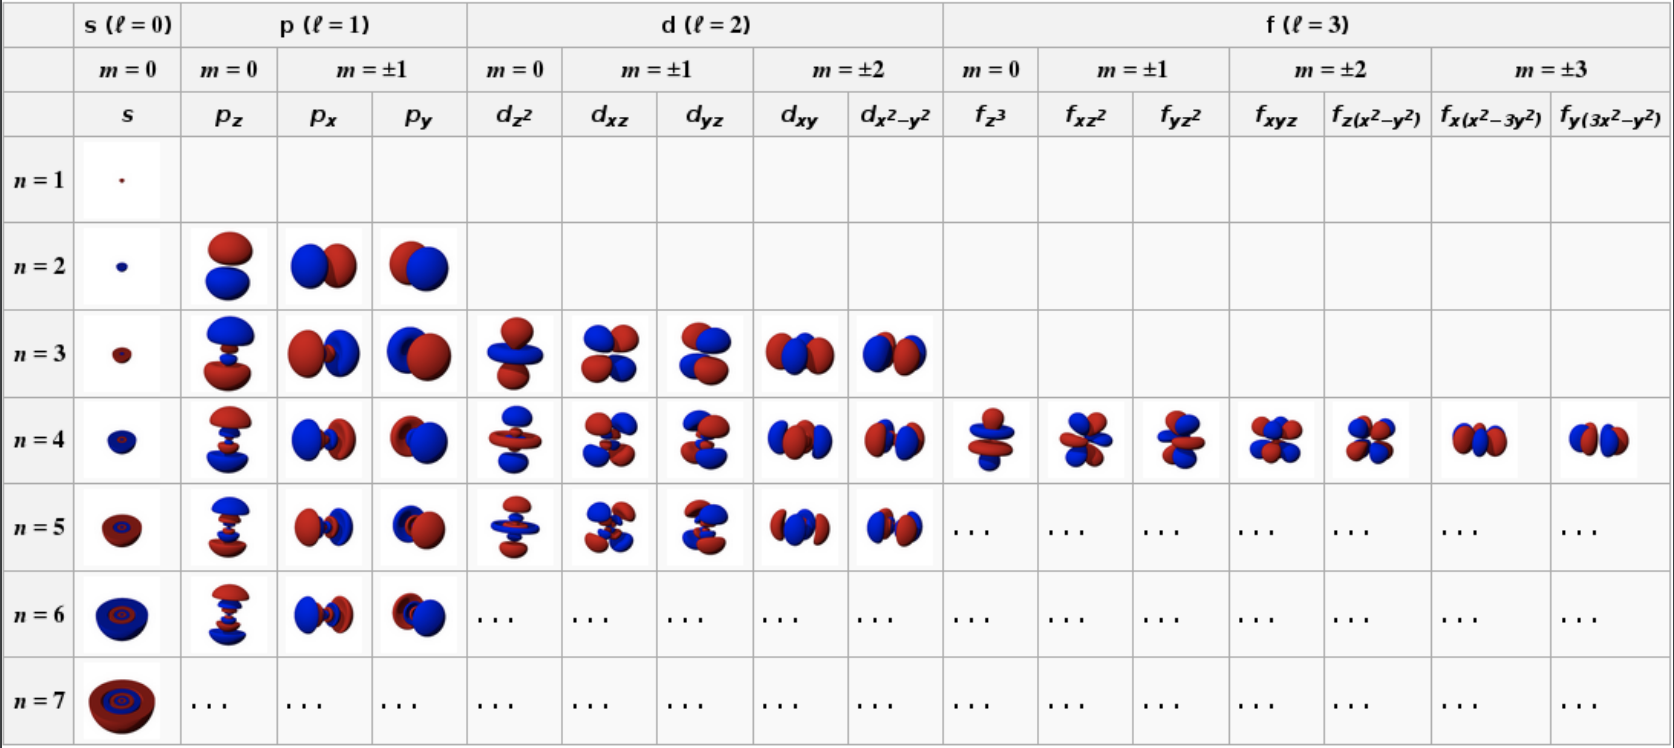
\includegraphics[scale=0.2]{HydrogenTable.png}
\end{center}
\begin{scriptsize}
    The $n$ value appears in the denominator of the exponential\\
    The $n$ value is the highest power of $r$ in the exponential plus 1
\end{scriptsize}
    \end{minipage}
};
\node[fancytitle, right=10pt] at (box.north west) {Hydrogen Wavefunction};

\end{tikzpicture}

%------------ Schrodinger Potential Barriers/Wells ---------------
\begin{tikzpicture}
\node [mybox] (box){%
    \begin{minipage}{0.45\textwidth}
\subtopic{Cartesian Harmonic Oscillator}
    \begin{tabular}{lp{8cm} l}
Wavefunction & $\psi_{n_x,n_y,n_z}(x,y,z)=H_{n_x}\brround{\frac{x}{b}}e^{-\frac{x^2}{2b^2}}H_{n_y}\brround{\frac{y}{b}}e^{-\frac{y^2}{2b^2}}H_{n_z}\brround{\frac{z}{b}}e^{-\frac{z^2}{2b^2}}$\\
Energy & $E_{n_x,n_y,n_z}=\brround{n_x+n_y+n_z+\frac{3}{2}}\hbar\sqrt{\frac{k}{m}},\ n\geq0$
\end{tabular}\\
\subtopic{Spherical Harmonic Oscillator}
    \begin{tabular}{lll}
Dimensionless Variables & $E=\eta\hbar\sqrt{\frac{k}{M}}$ & $r=b\rho$\\
Energy & $E_n=\brround{n+\frac{1}{2}}\hbar\sqrt{\frac{k}{M}}$ & $n>0$\\
Wavefunction & $\psi_{n\ell m}(r,\theta,\phi)=\frac{U_{n\ell}(r)}{r}Y_\ell^m(\theta,\phi)$\\
Solutions of $u_{\eta\ell}(\rho)$
\end{tabular}\\
\begin{tiny}
\begin{tabular}{r|ccccc}
$\eta=4+\frac{3}{2}$ & $\brround{\rho^5-5\rho^3+\frac{15}{4}\rho}e^{-\frac{\rho^2}{2}}$ & & $\brround{\rho^5-5\rho^3}e^{-\frac{\rho^2}{2}}$ & & $\rho^5e^{-\frac{\rho^2}{2}}$\\
$\eta=3+\frac{3}{2}$ & & $\brround{\rho^4-3\rho^2}e^{-\frac{\rho^2}{2}}$ & & $\rho^4e^{-\frac{\rho^2}{2}}$\\
$\eta=2+\frac{3}{2}$ & $\brround{\rho^3-\frac{3}{2}\rho}e^{-\frac{\rho^2}{2}}$ & & $\rho^3e^{-\frac{\rho^2}{2}}$\\
$\eta=1+\frac{3}{2}$ & & $\rho^2e^{-\frac{\rho^2}{2}}$\\
$\eta=0+\frac{3}{2}$ & $\rho e^{-\frac{\rho^2}{2}}$\\
\hline
 & $\ell=0$ & $\ell=1$ & $\ell=2$ & $\ell=3$ & $\ell=4$
\end{tabular}
\end{tiny}
    \end{minipage}
};
\node[fancytitle, right=10pt] at (box.north west) {3D Quantum Harmonic Oscillator};

\end{tikzpicture}


\end{multicols*}



\end{document}


% Topics covered from Mattison
% Relativity of space-time and relativistic particles
% Photon quantum properties
% Spectra, Bohr Model and X-rays
% Schrodinger's solutions for the following
    % Free particles in 1D and maybe 3D
    % Step potentials
    % Tunneling
    % Square well potentials
    % Harmonic oscillators
% Lasers and band-structures
% Write (but not derive or solve) spherical coordinate Schrodinger
% Recognize or use spherical harmonics (table provided)
% Recognize or use hydrogen wave functions (table provided)
% Harmonic oscillator wave functions (Hermite polynomials provided)